\documentclass[10pt]{article}
\usepackage[margin=1.05cm,top=0.8cm,bottom=0.8cm,columnsep=0.55cm]{geometry}
\usepackage[utf8]{inputenc}
\usepackage[T1]{fontenc}
\usepackage{lmodern}
\usepackage{microtype}
\usepackage{multicol}
\usepackage{booktabs}
\usepackage{xcolor}
\usepackage{hyperref}
\usepackage{tikz}
\usetikzlibrary{positioning,arrows.meta}

\definecolor{ucblue}{RGB}{0,51,102}
\hypersetup{colorlinks=true,urlcolor=ucblue,linkcolor=ucblue}
\setlength{\parindent}{0pt}
\setlength{\parskip}{2.5pt}
\pagestyle{empty}
\newcommand{\head}[1]{\textbf{\color{ucblue}#1}\hspace{0.4em}}
\newcommand{\VideoURL}{\href{https://drive.google.com/file/d/1ovemshyIkbVYasXr7zaFDXIrdrHN7OH5/view}{Google Drive}}

\begin{document}

\begin{center}
{\Large\bfseries\color{ucblue} SQL4Business: Deliverable 2}\\[2pt]
{\small Generative Artificial Intelligence (580694), Universidad de Concepci\'on}\\[1pt]
{\small Aredhel Jim\'enez, Bryan Riquelme, Guido Salazar, Vicente So\~nez}\\[1pt]
{\small C\'odigo: \href{https://github.com/aredhel-jmze/Asistente-SQL-4-Business}{github.com/aredhel-jmze/Asistente-SQL-4-Business}
\quad$\vert$\quad Video: \VideoURL}
\end{center}

\vspace{-2pt}
\begin{center}
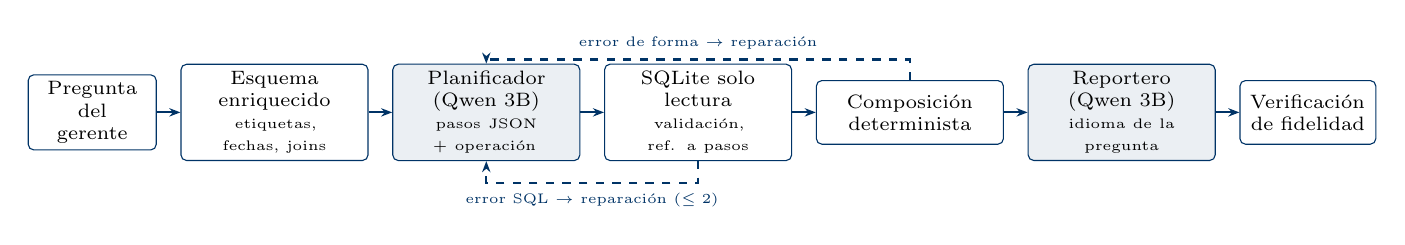
\begin{tikzpicture}[
  box/.style={draw=ucblue, rounded corners=2pt, align=center, font=\scriptsize, inner sep=2.5pt, minimum height=2.3em, text width=#1},
  box/.default=2.2cm,
  llm/.style={box=#1, fill=ucblue!8}, llm/.default=2.2cm,
  arrow/.style={-{Stealth[length=4pt]}, thick, ucblue}, node distance=0.3cm]
  \node[box=1.45cm] (q) {Pregunta del\\gerente};
  \node[box, right=of q] (s) {Esquema enriquecido\\{\tiny etiquetas, fechas, joins}};
  \node[llm, right=of s] (p) {Planificador (Qwen 3B)\\{\tiny pasos JSON + operaci\'on}};
  \node[box, right=of p] (x) {SQLite solo lectura\\{\tiny validaci\'on, ref. a pasos}};
  \node[box, right=of x] (c) {Composici\'on\\determinista};
  \node[llm, right=of c] (r) {Reportero (Qwen 3B)\\{\tiny idioma de la pregunta}};
  \node[box=1.55cm, right=of r] (f) {Verificaci\'on\\de fidelidad};
  \foreach \a/\b in {q/s, s/p, p/x, x/c, c/r, r/f} \draw[arrow] (\a) -- (\b);
  \draw[arrow, dashed] (x.south) -- ++(0,-0.28) -| node[pos=0.25, below, font=\tiny] {error SQL $\rightarrow$ reparaci\'on ($\leq 2$)} (p.south);
  \draw[arrow, dashed] (c.north) -- ++(0,0.26) -| node[pos=0.25, above, font=\tiny] {error de forma $\rightarrow$ reparaci\'on} (p.north);
\end{tikzpicture}
\end{center}
\vspace{-6pt}

\begin{multicols}{2}
\small

\head{Tarea, falla y modelo.} Sin cambios respecto del Deliverable 1: responder preguntas de
negocio puntuales y combinadas ejecutando el SQL necesario y reportando solo cifras fieles a
los resultados. Con prompting directo, los tres candidatos obtuvieron 0/5 en preguntas combinadas
(a\~nos inventados, etiquetas traducidas, dialectos de otros motores, una sola consulta para una
pregunta de varios valores). Nos comprometemos con \texttt{Qwen/Qwen2.5-Coder-3B-Instruct}
(revisi\'on \texttt{488639f}, NF4 de 4 bits, c\'omputo bf16, decodificaci\'on greedy, Colab T4):
es el menor candidato y empat\'o el mejor baseline propio (46.7\%); Qwen-7B obtuvo 33.3\% y
Llama-8B tambi\'en 46.7\%, con m\'as par\'ametros y acceso restringido.

\head{Intervenci\'on.} Cada componente ataca un error diagnosticado. El esquema enriquecido
entrega las etiquetas exactas, el rango de fechas y las llaves de uni\'on (etiquetas traducidas,
a\~nos inventados). El planificador descompone la pregunta en pasos SQL y nombra una operaci\'on;
el c\'odigo, no el modelo, calcula crecimiento, participaci\'on, comparaci\'on y
filtro con ranking (preguntas combinadas, aritm\'etica mental). SQLite se ejecuta en solo lectura;
los errores de validaci\'on o de forma vuelven al planificador hasta dos veces. Un paso posterior
puede leer uno anterior (\texttt{FROM step\_1}), que se expande como CTE. El reportero escribe en
el idioma de la pregunta, y la verificaci\'on acepta una cifra solo si coincide con la respuesta
verificada o con la evidencia a la precisi\'on escrita, y controla la direcci\'on del cambio.

\head{Evaluaci\'on.} Set oficial: las 15 preguntas del Deliverable 1 (10 puntuales, 5 combinadas),
usadas durante el desarrollo, por lo que es in-sample. Set externo: 12 par\'afrasis (5/7) con la
misma referencia, escritas en una auditor\'ia y no usadas para el dise\~no. Todos los sistemas
reciben las mismas entradas y criterios: \textit{sql} es el criterio del Deliverable 1 (cada
resultado de referencia se produce exactamente); \textit{answer} revisa la respuesta final, sin
importar c\'omo se obtuvo; \textit{report} y \textit{e2e} (respuesta y reporte correctos) se
aplican a la soluci\'on. El baseline es el prompt del Deliverable 1, literal; la estrategia
alternativa solo le agrega el esquema enriquecido.

\head{Resultados (tabla inferior).} La soluci\'on responde 11/15 preguntas oficiales y 10/12
externas, frente a 8/15 y 5/12 del baseline; en combinadas, 2/5 y 5/7 frente a 1/5 y 2/7.
Responde y reporta fielmente en 10/15 y 10/12. El esquema enriquecido explica la mayor parte de
la mejora en puntuales (9/10 respuestas oficiales); la descomposici\'on suma las combinadas.
Costo en la T4: 16.3\,s por pregunta frente a 6.2\,s del baseline.

\head{Desviaciones declaradas.} (1) La primera versi\'on (17-09) eleg\'ia la operaci\'on con
palabras copiadas de las 5 preguntas combinadas y vetaba otros planes: 12/15 in-sample, pero 0/7
en par\'afrasis combinadas. Se elimin\'o. (2) Esa versi\'on usaba adem\'as un nuevo prompt de
baseline en ingl\'es (40\%); se restituy\'o el prompt del D1. (3) Se agreg\'o la m\'etrica
\textit{answer} porque el criterio \textit{sql} rechaza respuestas correctas de una sola consulta
(el baseline responde bien q14). (4) No se aplic\'o el fine-tuning QLoRA previsto en el D1.
(5) La primera corrida de esta versi\'on (v2) descart\'o reportes en texto plano por no ser JSON;
v3 solo cambia el formato de salida del reportero, y su SQL y respuestas son id\'enticos a v2 en
27/27 preguntas.

\head{Caso de falla: q09.} El planificador filtra con \texttt{strftime('\%Y-\%m', sale\_date)
BETWEEN '2026-03-01' AND '2026-05-31'}. Comparar \texttt{'2026-03'} con una fecha completa deja
fuera marzo y junio, por lo que el c\'odigo calcula un crecimiento de 70.06\% en vez de 60.13\%.
El SQL es v\'alido, el resultado es un solo n\'umero y el reporte es fiel a \'el, de modo que ni
la validaci\'on, ni la reparaci\'on, ni la verificaci\'on detectan el error: revisan forma y
cifras, no el significado de un predicado. En q10 el modelo vuelve a usar
\texttt{strftime('\%Q')} pese al mensaje de error, y en q09-p (externa) planifica un solo paso,
por lo que el crecimiento nunca se calcula; su reporte inventa 26\%, 10\% y 12\%, y la
verificaci\'on lo rechaza.

\head{L\'imites.} Los resultados oficiales son in-sample y ambos sets son peque\~nos (27
preguntas, datos sint\'eticos). La verificaci\'on controla cifras, no su atribuci\'on: en q11
acepta 488 presentado como total, y en q14-p un id de producto tomado de un paso. Adem\'as es
conservadora: rechaza ``paso 1'' en q13. Cuando el planificador elige \textit{direct} para una
pregunta combinada, la respuesta depende de una sola consulta. Los reintentos rara vez corrigen
un plan (sesgos fuertes del modelo).

\head{Reproducci\'on.} \texttt{notebooks/deliverable2\_demo.ipynb} en una T4 de Colab
(\textit{Run all}, unos 25 min) clona el repositorio, corre la demo del video y la evaluaci\'on,
y escribe \texttt{results/deliverable2\_v3.json} y la tabla inferior; no requiere subir archivos
ni tokens.
\end{multicols}

\vspace{-4pt}
\begin{center}
\footnotesize
\begin{tabular}{@{}llccccc@{}}
\toprule
& & \multicolumn{3}{c}{\textbf{Set oficial (in-sample)}} & \multicolumn{2}{c}{\textbf{Paráfrasis (held-out)}} \\
\cmidrule(lr){3-5}\cmidrule(l){6-7}
\textbf{Sistema} & \textbf{Métrica} & Puntual & Combinada & Total & Puntual & Combinada \\
\midrule
Prompt directo (baseline D1) & sql & 7/10 & 0/5 & 7/15 & 3/5 & 0/7 \\
 & answer & 7/10 & 1/5 & 8/15 & 3/5 & 2/7 \\
\addlinespace
Prompt directo + esquema enriquecido & sql & 8/10 & 0/5 & 8/15 & 4/5 & 0/7 \\
 & answer & 9/10 & 1/5 & 10/15 & 4/5 & 4/7 \\
\addlinespace
Solución estructurada & sql & 9/10 & 2/5 & 11/15 & 5/5 & 3/7 \\
 & answer & 9/10 & 2/5 & 11/15 & 5/5 & 5/7 \\
 & report & 8/10 & 4/5 & 12/15 & 5/5 & 6/7 \\
 & e2e & 8/10 & 2/5 & 10/15 & 5/5 & 5/7 \\
\bottomrule
\end{tabular}

\end{center}

\end{document}
